\documentclass[a4paper]{article}
\usepackage{amsmath}
\usepackage{amssymb}
\usepackage{xcolor}
\usepackage{amsthm}
\usepackage{dsfont}
\usepackage{graphicx}
\usepackage{subcaption}
\usepackage{hyperref}
\usepackage{datetime}
\usepackage{outlines}
\usepackage[round]{natbib}   % omit 'round' option if you prefer square brackets

\usepackage[margin=3.8cm, top=3cm, bottom=3cm]{geometry}

\usepackage{matlab-prettifier}

\newdateformat{monthyeardate}{\monthname[\THEMONTH] \THEYEAR}

\newcommand{\newmarkedtheorem}[1]{%
  \newenvironment{#1}
    {\pushQED{\qed}\csname inner@#1\endcsname}
    {\popQED\csname endinner@#1\endcsname}%
  \newtheorem{inner@#1}%
}

\theoremstyle{definition}
%\newtheorem{eg}{Example}[section]
\newmarkedtheorem{eg}{Example}[section]
\newtheorem{observation}{Observation}[section]
\newtheorem{define}{Definition}[section]
\theoremstyle{plain}
\newtheorem{proposition}{Proposition}[section]
\newtheorem{theorem}{Theorem}[section]
\newtheorem{assump}{Assumption}
\newtheorem{remark}{Remark}

\author{Jeroen van Riel}
\date{\monthyeardate\today}
\title{Explicit Trajectory Generation}

\begin{document}

\begin{figure}
  \centering
  \makebox[\textwidth][c]{% wider than textwidth
    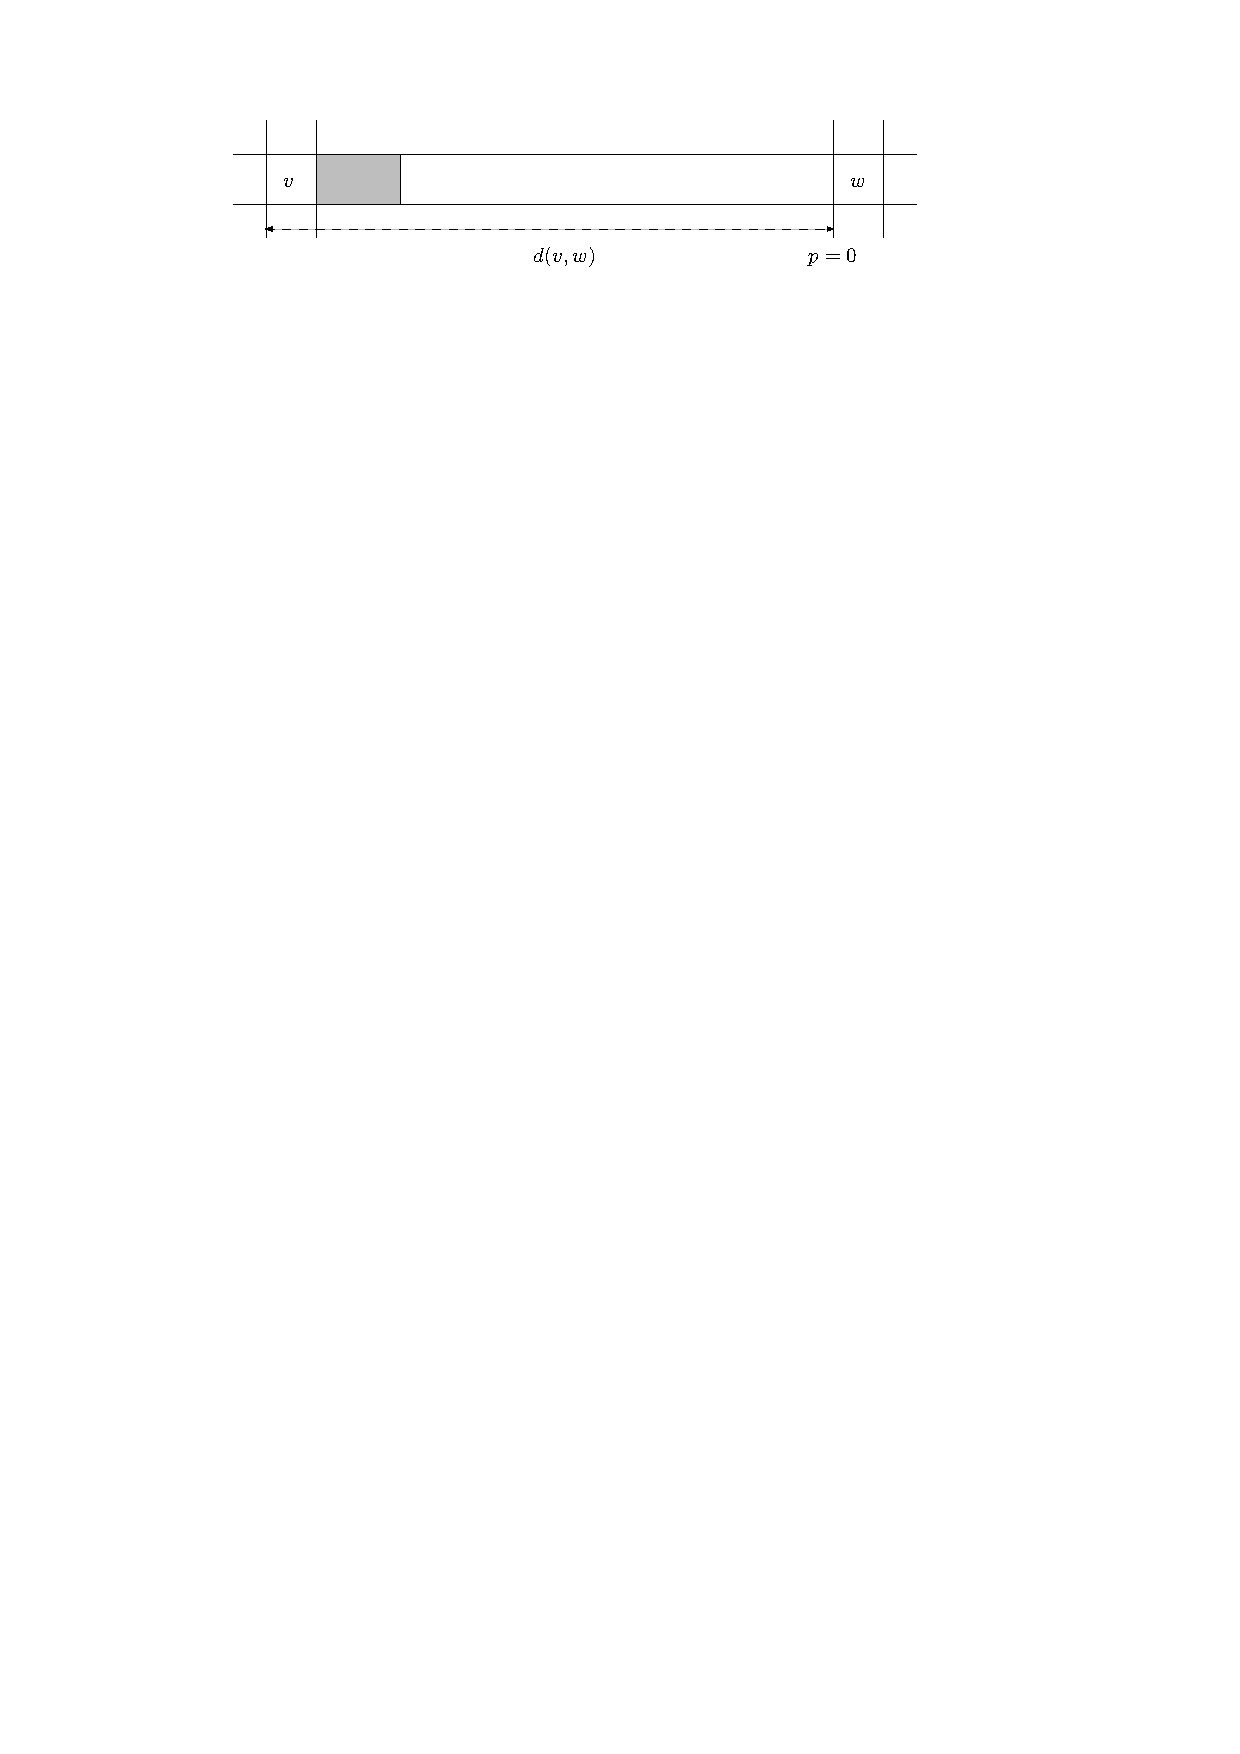
\includegraphics[width=1.0\textwidth]{figures/motion/tandem}
  }
  \caption{Tandem of two intersections $v$ and $w$ with lane of length $d(v,w)$.
    The grey rectangle represents some vehicle that just left intersection $v$,
    so it has maximum speed and is allowed to decelerate from here on.}
  \label{fig:tandem}
\end{figure}

\section{Tandem of intersections}

% motivation for model
We need to take into account the fact that a lane between two consecutive
intersections has finite capacity for vehicles, in order to model possible
blocking effects, also known as \textit{spillback}. The capacity of a lane is intimately
related to trajectories of vehicles, which we first want to understand better.
We have been using an optimal control formulation with the objective that keeps
the vehicles as close as possible to the next intersection at all times
(\texttt{MotionSynthesize}). This problem can be solved using direct
transcription, which works well enough if we just want to simulate the behavior
of the system. However, we believe that it is possible to explicitly formulate
the optimal control. Below, we will explain how to compute trajectories
corresponding to those obtained by direct transcription, but without using time
discretization. Our approach may be considered an \textit{ansatz}, because
proving that this is indeed the optimal control would need to invoke some kind
of sufficiency theorem and, perhaps more importantly, there are still some cases
in which the implementation breaks down.

% define tandem model
We start with the simplest extension of the single intersection model by
considering two intersections in tandem, as illustrated in
Figure~\ref{fig:tandem}. Let $v$ denote the left intersection and $w$ the right
intersection and assume that vehicles drive from left to right. Let the length
and width of a vehicle $i$ be denoted by $L_{i}$ and $W_{i}$, respectively. We
measure the position of a vehicle at the front bumper and we let position $x=0$
be at the stopline of intersection $v$. We denote the position of the stopline
at $w$ by $x=x_{f}=d(v,w)$. To simplify the following discussion, we assume that all
vehicles have the same dimensions.

\begin{assump}
  \label{assump1}
  All vehicles have the same length $L_{i} = L$ and width $W_{i} = W$.
\end{assump}

Now assume that some vehicle is scheduled to cross $v$ at time $t=0$ and to
cross $w$ at some time $t_{f}$. Let $y(t)$ denote the trajectory of the
predecessor, assuming there is one. In order to keep the vehicle as close to $w$
as possible at every time, we can generate a trajectory by solving the optimal
control problem
\begin{equation}
  \label{eq:optimal_control}
  \begin{aligned}
  \max_{x}    \quad & \int_{t=0}^{t_{f}} x(t) dt \\
  \begin{alignedat}{2}\text{s.t.}\\ {}\end{alignedat} \quad &\begin{alignedat}{2}
                     0 \leq \; &\dot{x}(t) \leq v_{\max} , \\
                     {-a_{\max}} \leq \; &\ddot{x}(t) \leq a_{\max} , \\
                    y(t) \leq \; & x(t) , \\
                    \end{alignedat} \\
                    &\begin{alignedat}[t]{2}
                    & x(0) = 0 , &&  x(t_{f}) = d(v,w) , \\
                    & \dot{x}(0) = v_{\max} , \;\; && \dot{x}(t_{f}) = v_{\max} .
                    \end{alignedat}
  \end{aligned}
\end{equation}
%
We believe that the optimal control $u(t) := \ddot{x}(t)$ satisfies
$u(t) \in \{-a_{\max}, 0, a_{\max}\}$ and there is a sequence of alternating
deceleration and acceleration periods, meaning that there is a sequence of
disjoint intervals
\begin{align*}
  (D_{1}, A_{1}, \dots, D_{n}, A_{n}) ,
\end{align*}
so that the optimal controller is given by
\begin{align*}
  u(t) = \begin{cases}
           {-a_{\max}} &\text{ if } t \in D_{k} \text{ for some } k , \\
           \phantom{-} a_{\max}   &\text{ if } t \in A_{k} \text{ for some } k , \\
           \phantom{-} \;\, 0 &\text{ otherwise. }
         \end{cases}
\end{align*}

\begin{figure}
  \centering
  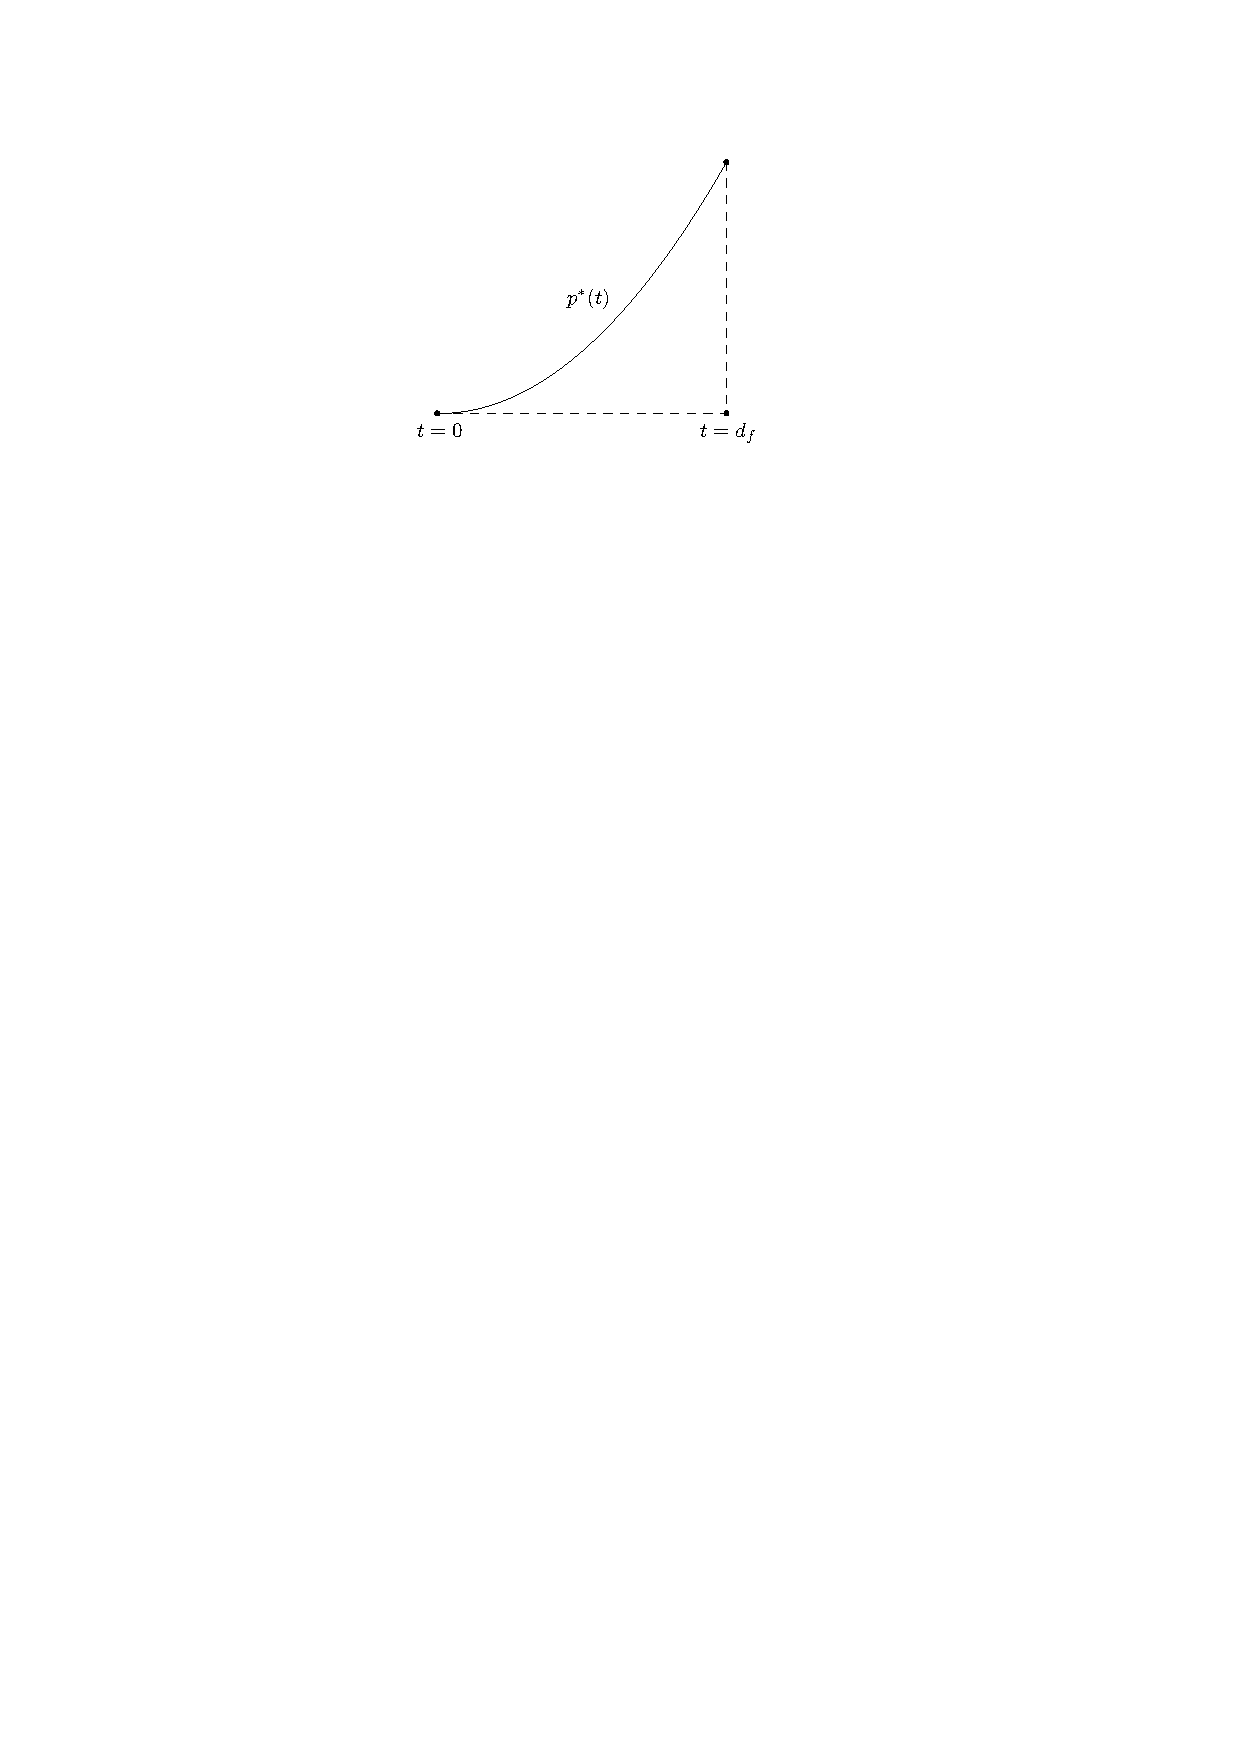
\includegraphics[scale=1]{figures/motion/acceleration}
  \caption{Full acceleration trajectory.}
  \label{fig:acceleration}
\end{figure}

\subsection{Single vehicle}
\label{sec:single}

We will start by assuming that the system contains a single vehicle, so that we
do not have to worry about keeping a safe distance to vehicle in front of it. We
will show how the bang-bang intervals, or \textit{bangs} for short, can be
obtained in this situation.
%
Without considering the boundary conditions, it follows from the vehicle
dynamics that the time it takes to fully accelerate from zero to maximum
velocity is given by
\begin{align*}
  T = v_{\max} / a_{\max} ,
\end{align*}
with corresponding trajectory $x^{*}$, given by
\begin{align*}
  x^{*}(t) = a_{\max} t^{2} / 2 \quad \text{ for }0 \leq t \leq T ,
\end{align*}
as illustrated in Figure~\ref{fig:acceleration}.
%
First, we introduce a transformation that will prove to be helpful. For position
$x$ at time $t$, we define the corresponding \textit{schedule time} by
\begin{align*}
  \bar{t}(t, x) := t - x / v_{\max} .
\end{align*}
This induces equivalence classes in time-position space, corresponding to lines
with slope $v_{\max}$. In the following, we will use a bar above a symbol when
dealing with schedule time.
%
For example, time duration $T$ translated to schedule time, is given by
\begin{align*}
  \bar{T} &= \bar{t}(T, x^{*}(T)) - \bar{t}(0, 0) = T / 2 .
\end{align*}

The crossing time of $v$ and $w$ in schedule time are given by $b = \bar{t}(0, 0)$
and $e = \bar{t}(t_{f}, x_{f})$, respectively.
%
Whenever $t_{f}$ is sufficiently large, it is clear that we need a full
deceleration bang and a full acceleration bang. Therefore, in schedule time,
this would take $2 \bar{T}$ time.
%
However, for smaller $t_{f}$, time of deceleration and acceleration need to
decrease equally. Therefore, writing $(x)^{+}$ for $\max(x, 0)$, the remaining
amount of schedule time in which the vehicle is stopped is given by
\begin{align*}
  \bar{d}_{s} = {(e - b - 2\bar{T})}^{+}
\end{align*}
and the length of each bang is
\begin{align*}
  \bar{d}_{b} = (e - b - \bar{d}_{s}) / 2 ,
\end{align*}
so that the bangs are given by
\begin{align*}
  \bar{D} = (b, b + \bar{d}_{b}) , \\
  \bar{A} = (e - \bar{d}_{b}, e) .
\end{align*}
The corresponding trajectory are shown in Figure~\ref{fig:single_trajectory}.


\begin{figure}
  \centering
\begin{subfigure}{0.4\textwidth}
    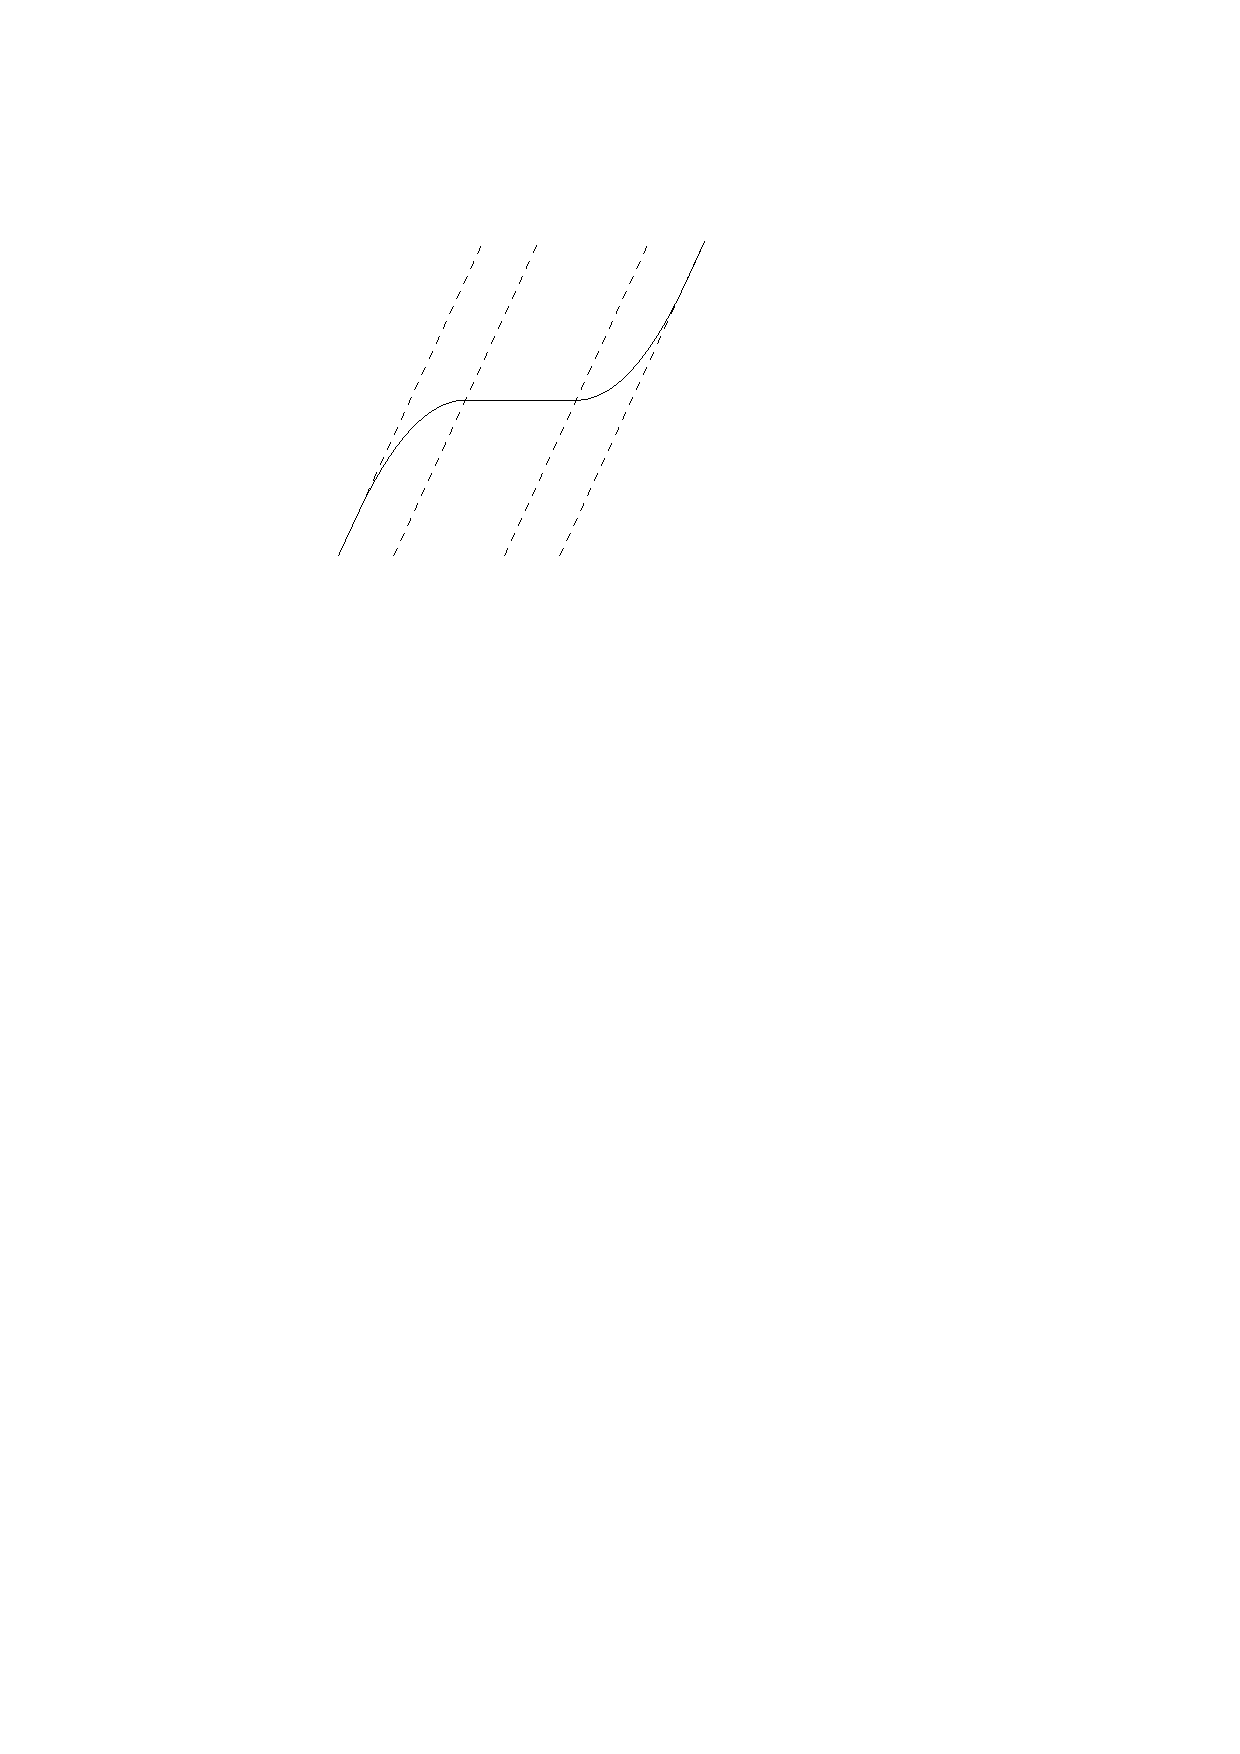
\includegraphics[scale=1]{figures/motion/single_trajectory_split}
    \caption{Positive waiting time $\bar{t}_{s} > 0$.}
    \label{fig:single_trajectory_split}
\end{subfigure}
\hfill
\begin{subfigure}{0.3\textwidth}
    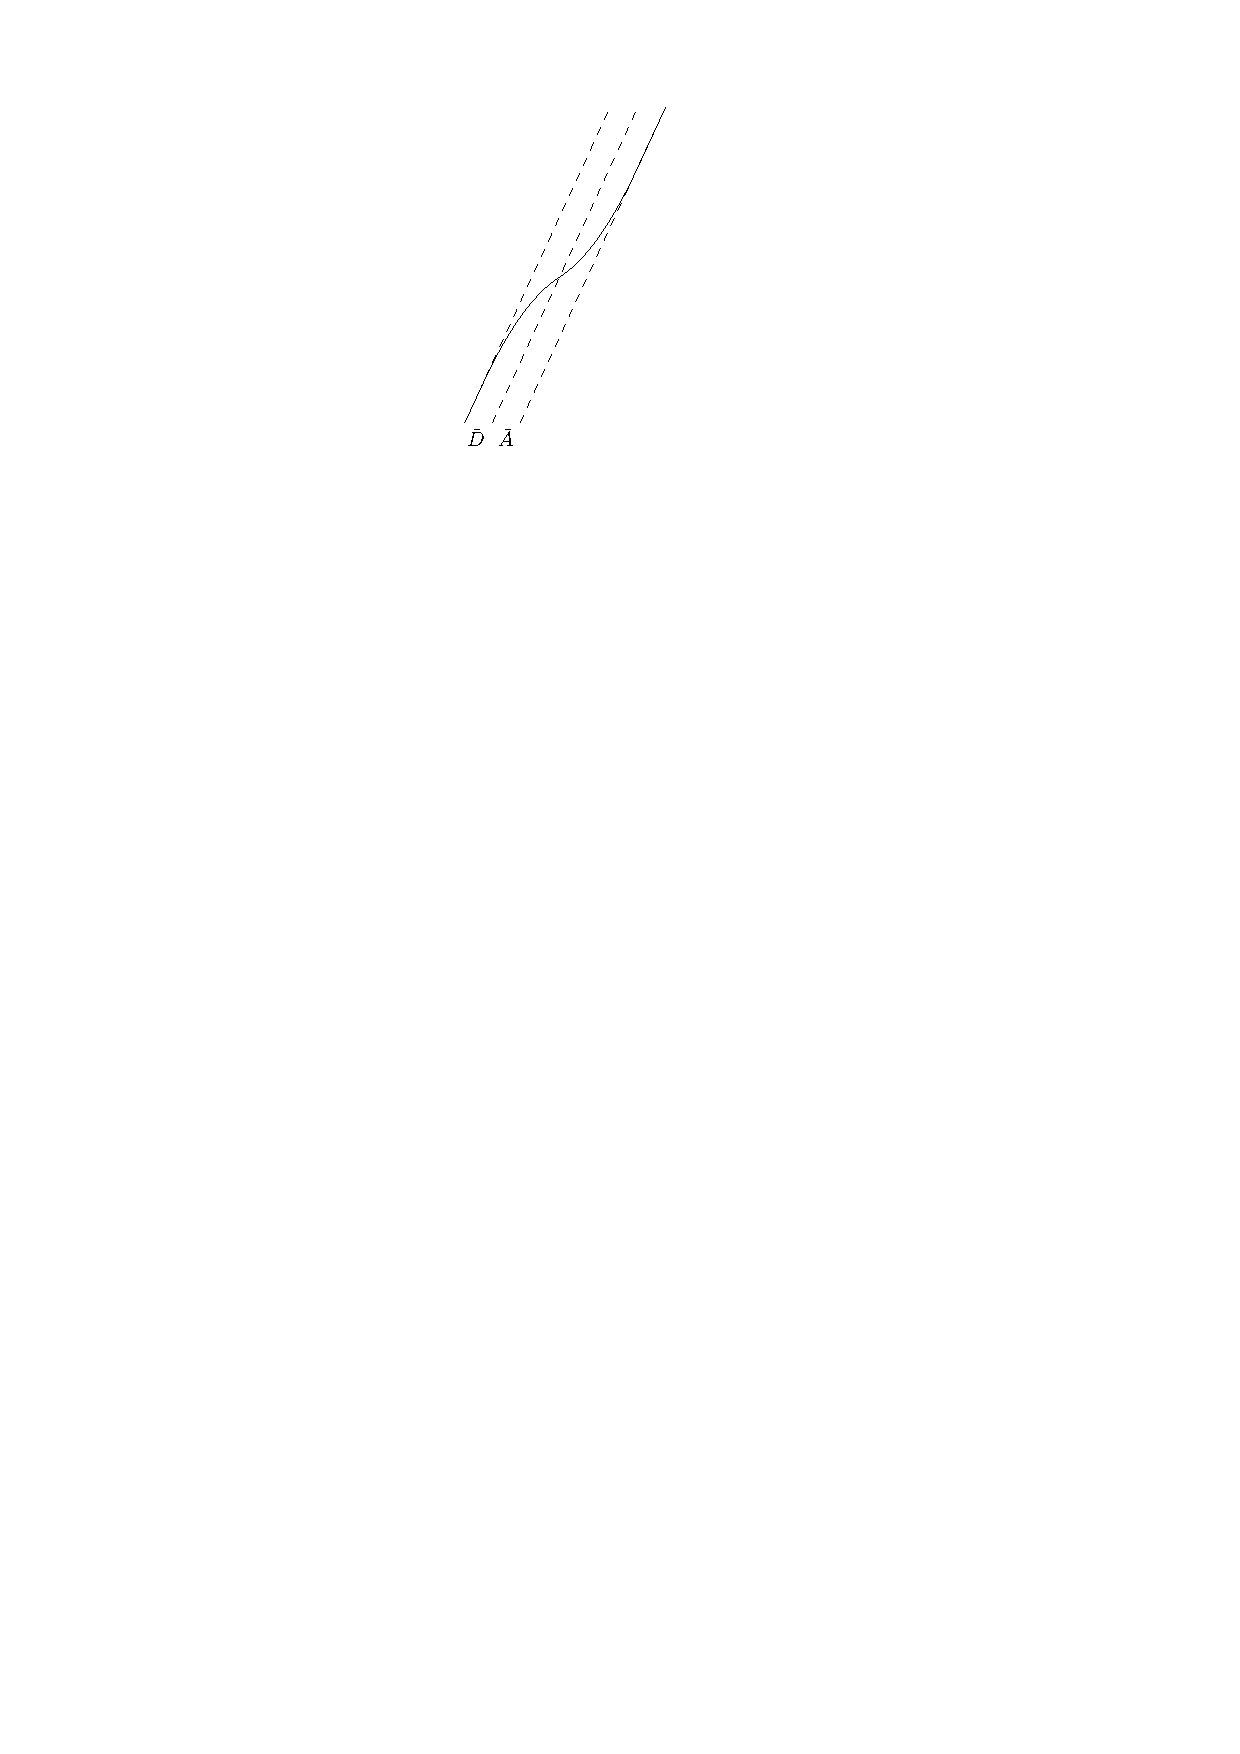
\includegraphics[scale=1]{figures/motion/single_trajectory_merged}
    \caption{Vehicle does not stop.}
    \label{fig:single_trajectory_merge}
\end{subfigure}
\caption{Shape of optimal trajectories $x(t)$ for a single (isolated) vehicle,
  in case the vehicle stops and waits for some time (a) and in case the vehicle
  does never come to a full stop (b). In each case, the deceleration bang
  $\bar{D}$ and acceleration bang $\bar{A}$ in schedule time are indicated by
  the dashed lines.}
  \label{fig:single_trajectory}
\end{figure}


Because the control $u(t)$ is not specified in terms of schedule scale, we need
to invert these bangs back to regular time.
%
Let $v_{c}$ denote the current velocity at the start of the bang and let
$\bar{d}$ denote the duration of the bang in schedule time. We first consider
the acceleration bang. Define $t_{0}= v_{c} / a_{\max}$ so that we have
$\dot{x}^{*}(t_{0}) = v_{c}$. Next, we find $t_{1}$ such that
$t_{0} \leq t_{1} \leq T$ and
\begin{align}
  \label{eq:regular}
   \bar{t}(t_{1}, x^{*}(t_{1})) - \bar{t}(t_{0}, x^{*}(t_{0})) = \bar{d} ,
\end{align}
such that the duration of the bang in regular time is given by $d = t_{1} - t_{0}$.
%
After some rewriting and substitution of the definitions of $x^{*}$ and
$\bar{t}$ in equation~\eqref{eq:regular}, we obtain the quadratic equation
\begin{align*}
  - \frac{a_{\max} t_{1}^{2}}{2 v_{\max}} + t_{1} - t_{0} + \frac{a_{\max} t_{0}^{2}}{2 v_{\max}} - \bar{d} = 0 ,
\end{align*}
for which we are interested in the solution
\begin{align*}
  t_{1} = T - \sqrt{T^{2} - 2T(t_{0} + \bar{d}) +t_{0}^{2}} .
\end{align*}
%
Similarly, we derive that the duration of a deceleration bang is given by
$d = t_{1} - t_{0}$ where $t_{0} = (v_{\max} - v_{c}) / a_{\max}$ and $t_{1}$ is
the solution to
\begin{align*}
  \bar{t}(t_{1}, -x^{*}(-t_{1})) - \bar{t}(t_{0}, -x^{*}(-t_{0})) = \bar{d} ,
\end{align*}
given by
\begin{align*}
  t_{1} = - T + \sqrt{T^{2} +2T(t_{0} + \bar{d}) + t_{0}^{2}} .
\end{align*}

We can now calculate the duration of the bangs in schedule time, but this does
not yet fix their time in a unique way. Due to the definition of schedule time,
we need to be careful whenever the velocity is $v_{\max}$, because the regular
time is not unique in this case. Therefore, we specify a \textit{target
  position} $x_{t}$ such that the start of the deceleration bang is given by
\begin{align*}
  b + (x_{t} - x^{*}(T)) / v_{max} .
\end{align*}
This ensures that the vehicle has enough distance to $w$ to accelerate, in case
it stops.


\subsection{Multiple vehicles}

\begin{figure}
  \centering
  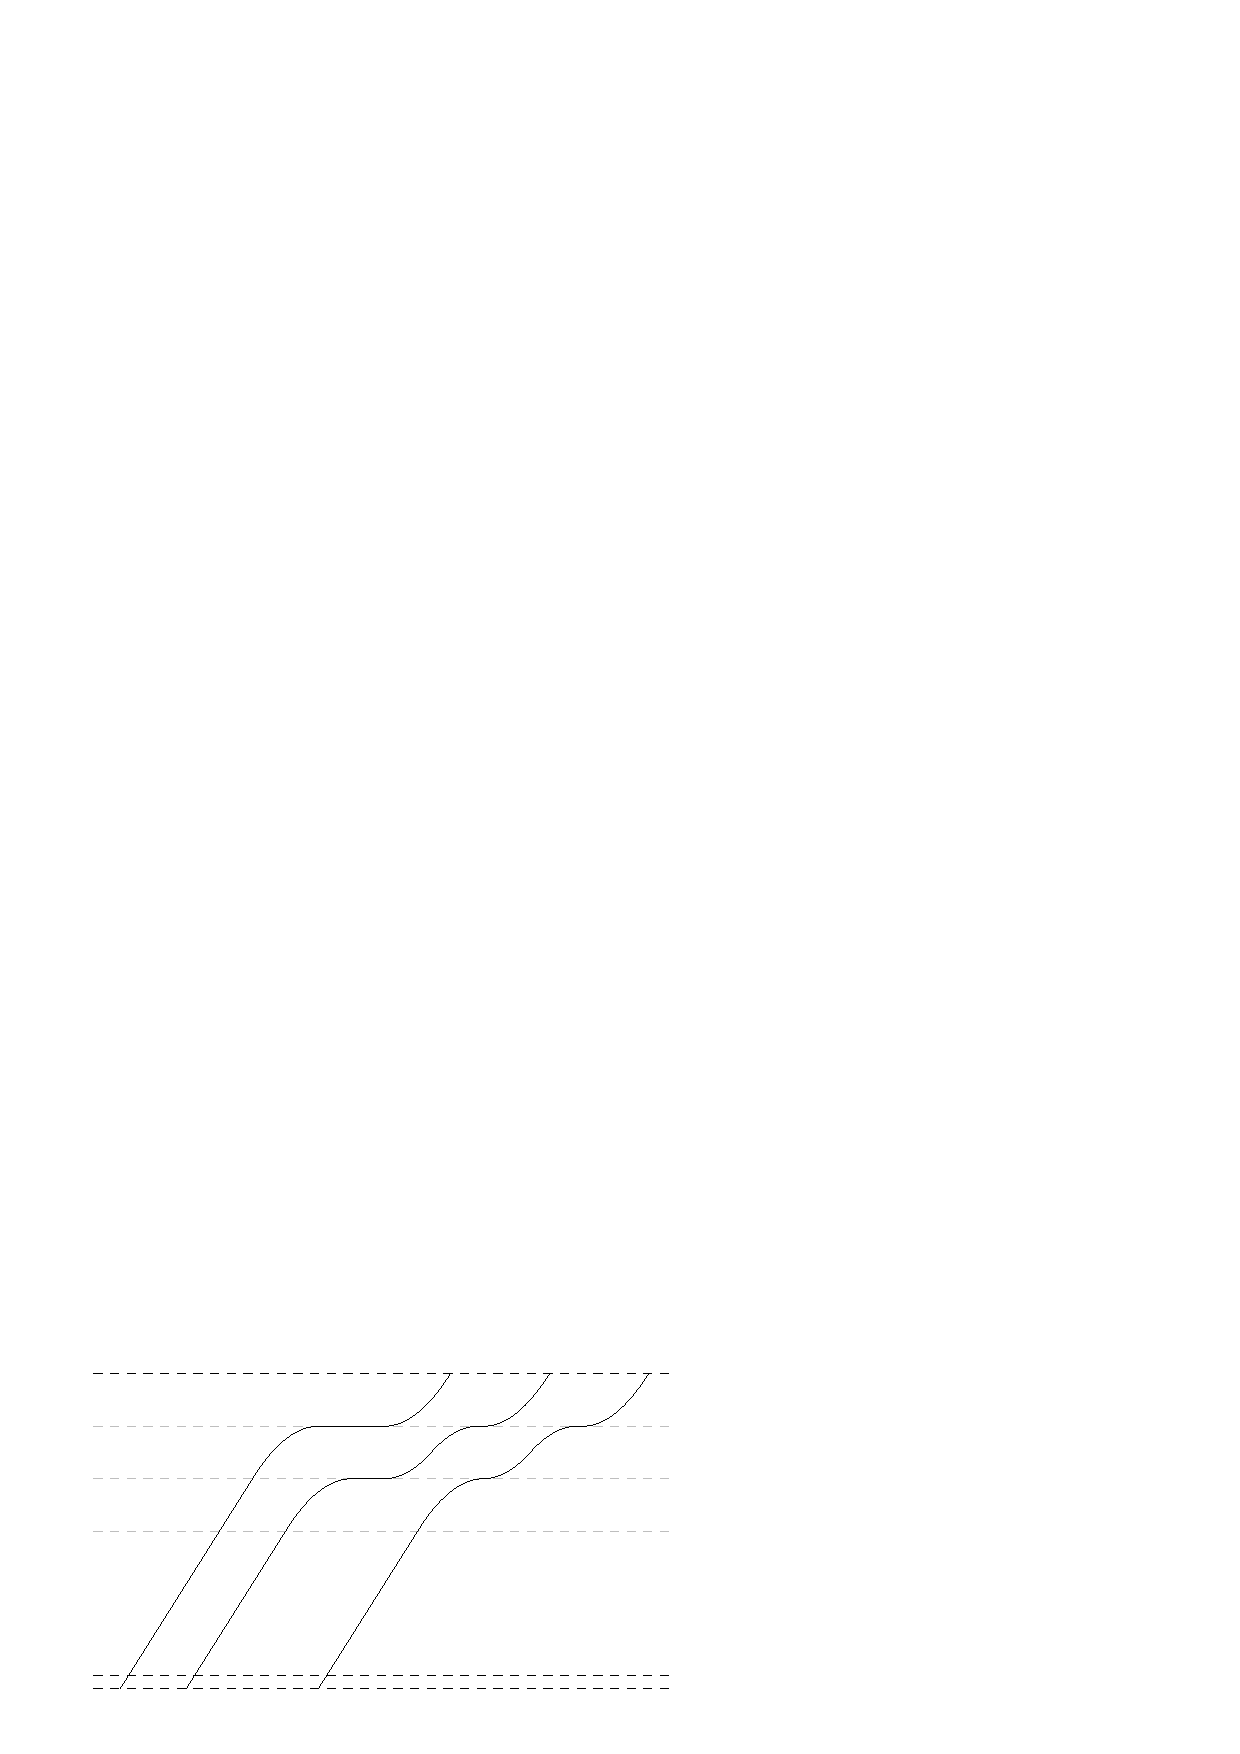
\includegraphics[scale=1.0]{figures/motion/buffer}
  \caption{Optimal trajectories displaying the start-stop queueing behavior. The
    waiting positions are indicated by the grey dashed lines. The bottom two
    horizontal dashed lines represent intersection $v$.}
  \label{fig:buffering}
\end{figure}

We will now consider the case when the system contains multiple vehicles. Now,
we need to take into account the safe following constraints. This also causes
additional \textit{buffer constraints} to the crossing time scheduling problem,
since the lane only provides space for a limited number of vehicles, which we
investigate in Section~\ref{sec:capacity}. For now, assume we have a feasible
crossing time schedule, that satisfies the buffer constraints.

Consider the optimal solution in Figure~\ref{fig:buffering}. Observe that all
vehicles undergo some start-stop phases. Furthermore, there are some fixed
positions where vehicles will come to a full stop, to which we refer as
\textit{waiting positions}. Recall that $L$ is the minimal distance between two
consecutive vehicles. From a waiting position, we move to the next waiting
position that is exactly $L$ units further on the lane.
%
We will now describe such a start-stop trajectory of a single vehicle, without
considering safe following constraints, see Figure~\ref{fig:start-stop}.
%
By symmetry of the control constraints, the vehicle moves the same distance
during both acceleration and deceleration. Furthermore, we need zero velocity at
the start and end of such trajectory. Hence, it is clear that the duration
$d_{n}$ of acceleration and deceleration need to be the same.
%
Assume for now that full acceleration/deceleration is not required, which is the
case whenever we have $L < 2 x^{*}(T)$. Therefore, $d_{n}$ must satisfy
$L = 2x^{*}(d_{n})$, so we obtain
\begin{align*}
d_{n} = \sqrt{L / a_{\max}} ,
\end{align*}
which corresponds to a duration in schedule time of
\begin{align*}
  \bar{d_{n}} = \bar{t}(t_{m}, L/2) = t_{m} - \frac{L}{2 v_{\max}} .
\end{align*}

\begin{figure}
  \centering
  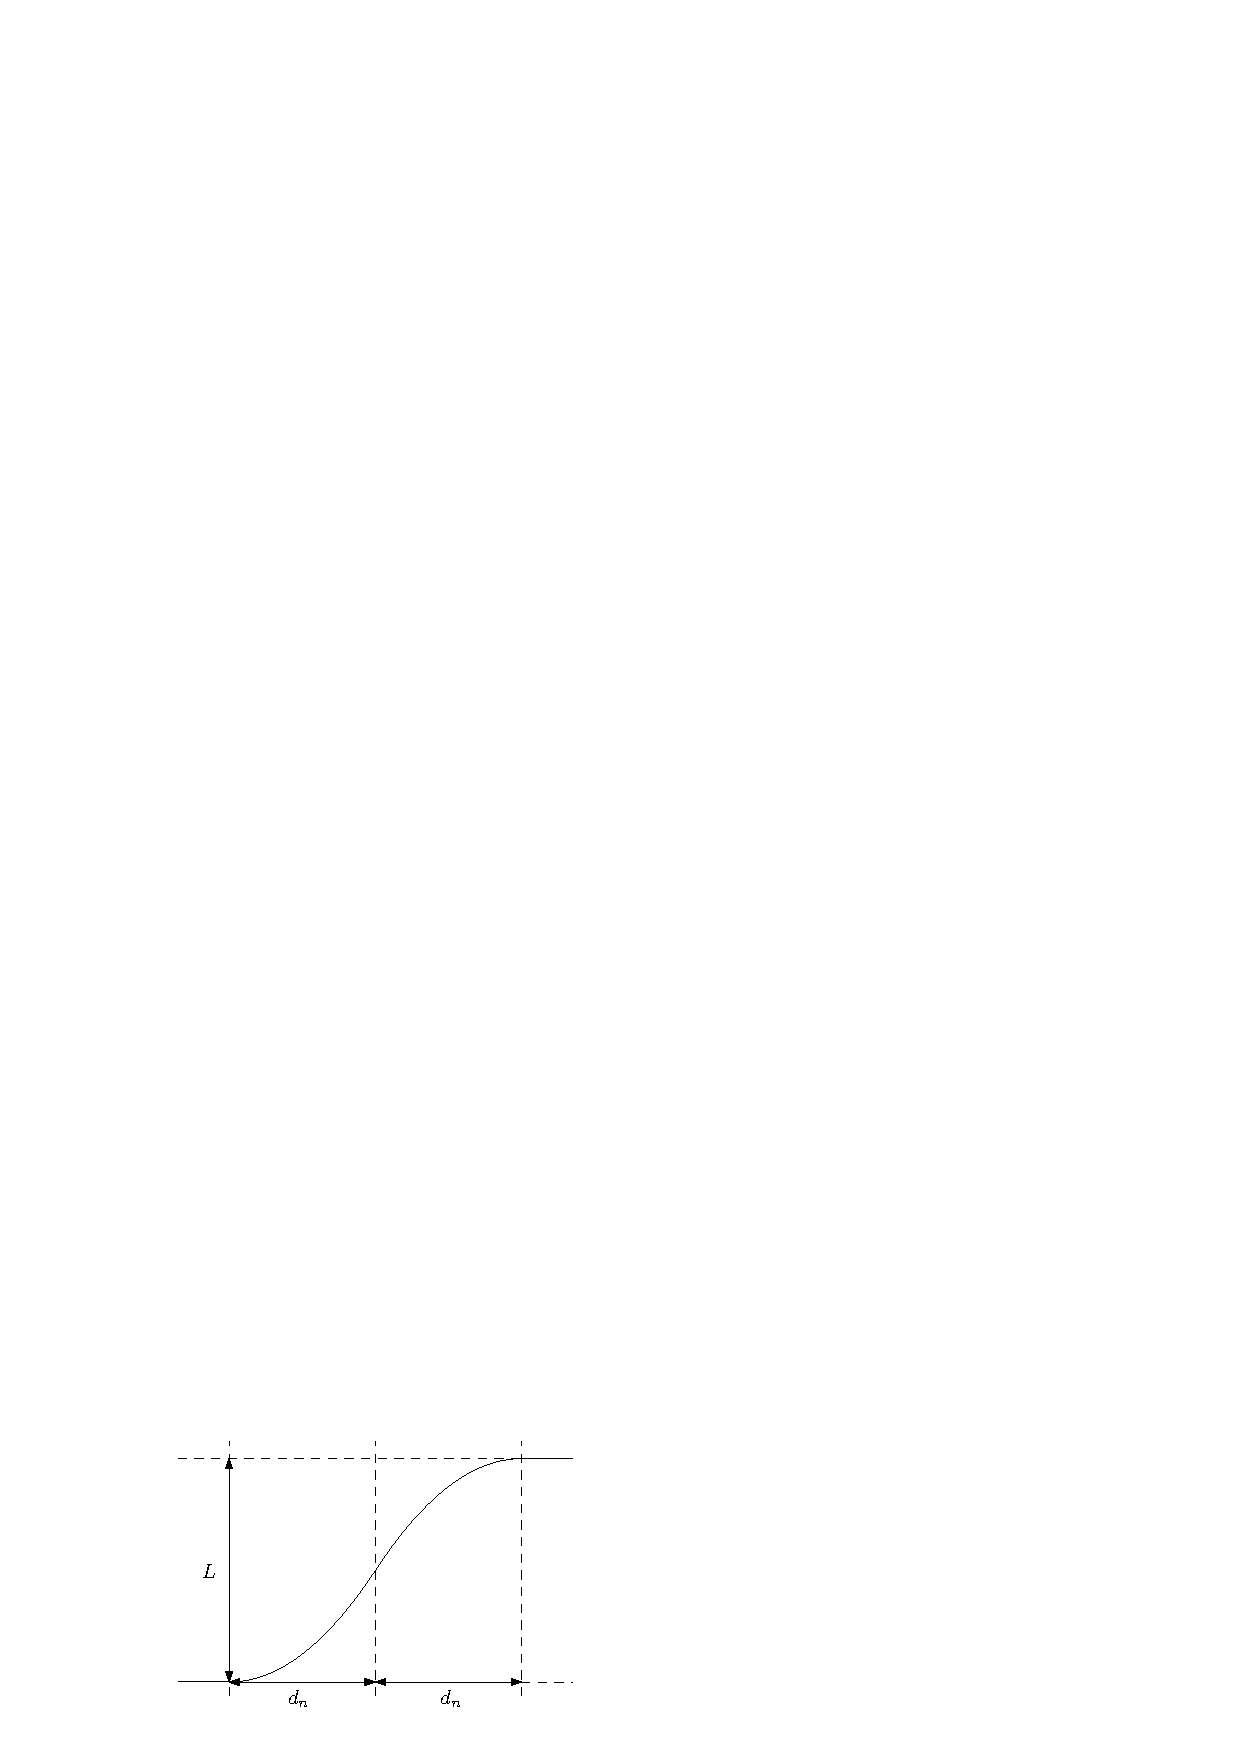
\includegraphics[scale=1.0]{figures/motion/start_stop_trajectory}
  \caption{Shape of the start-stop trajectory of a single isolate vehicle moving
    forward from the current waiting position to the next waiting position.}
  \label{fig:start-stop}
\end{figure}

We will now show how to construct the sequence of bangs in schedule time, given
the sequence of bangs in schedule time of the preceding vehicle. In general, we
observe that the the bangs of the preceding vehicle introduce additional pairs
of bangs corresponding to start-stop trajectories, apart from the first
deceleration and last acceleration that were also present in the single isolated
vehicle case.

We only need the start of the acceleration bangs of the preceding vehicle in
schedule time, which we denote by $\bar{t}_{1}, \dots, \bar{t}_{n}$. For every
$\bar{t}_{i}$, we introduce a pair of start-stop bangs at time
$\bar{t}_{i} + L / v_{\max}$.
%
Furthermore, we have an initial deceleration at $\bar{D}_{0} = [a, a + \bar{T}]$ and the final
acceleration at $\bar{A}_{f} = [y - \bar{T}, y]$.
%
This results in some sequence of bangs in schedule time
\begin{align*}
  (\bar{D}_{0}, \bar{A}_{1}, \bar{D}_{1}, \dots, \bar{A}_{n}, \bar{D}_{n}, \bar{A}_{f}) .
\end{align*}
Note that these bangs are not necessarily disjoint, so we \textit{merge} them in
the following simple way. Merging two intervals $[t_{0}, t_{1}]$ and
$[t_{2}, t_{3}]$ with $t_{1} > t_{2}$, results in the intervals $[t_{0}, t_{m}]$
and $[t_{m}, t_{3}]$ with $t_{m} = (t_{1} + t_{2})$.


Now that we have a sequence of disjoint bangs, we still need to translate them
back to the regular time scale, which can be done using the formulas from
Section~\ref{sec:single}.
%
We assume that the velocity never reaches $v_{\max}$. If this assumption does
not hold, the whole trajectory could be ``shifted up'' in the graph, which would
decrease the objective, so the trajectory would not be optimal. We keep track of
the current time $t_{c}$ and velocity $v_{c}$. For each next bang $\bar{A}$ or
$\bar{D}$ in the sequence, we compute the duration $d$ in regular time and
update $v_{c} \leftarrow v_{c} \pm a_{\max} d$ accordingly and set
$t \leftarrow t + d$. This way, we obtain the sequence of bangs in regular time,
which completely defines the controller.


\subsection{Lane capacity}\label{sec:capacity}

\begin{figure}[b]
  \centering
  \makebox[\textwidth][c]{% wider than textwidth
    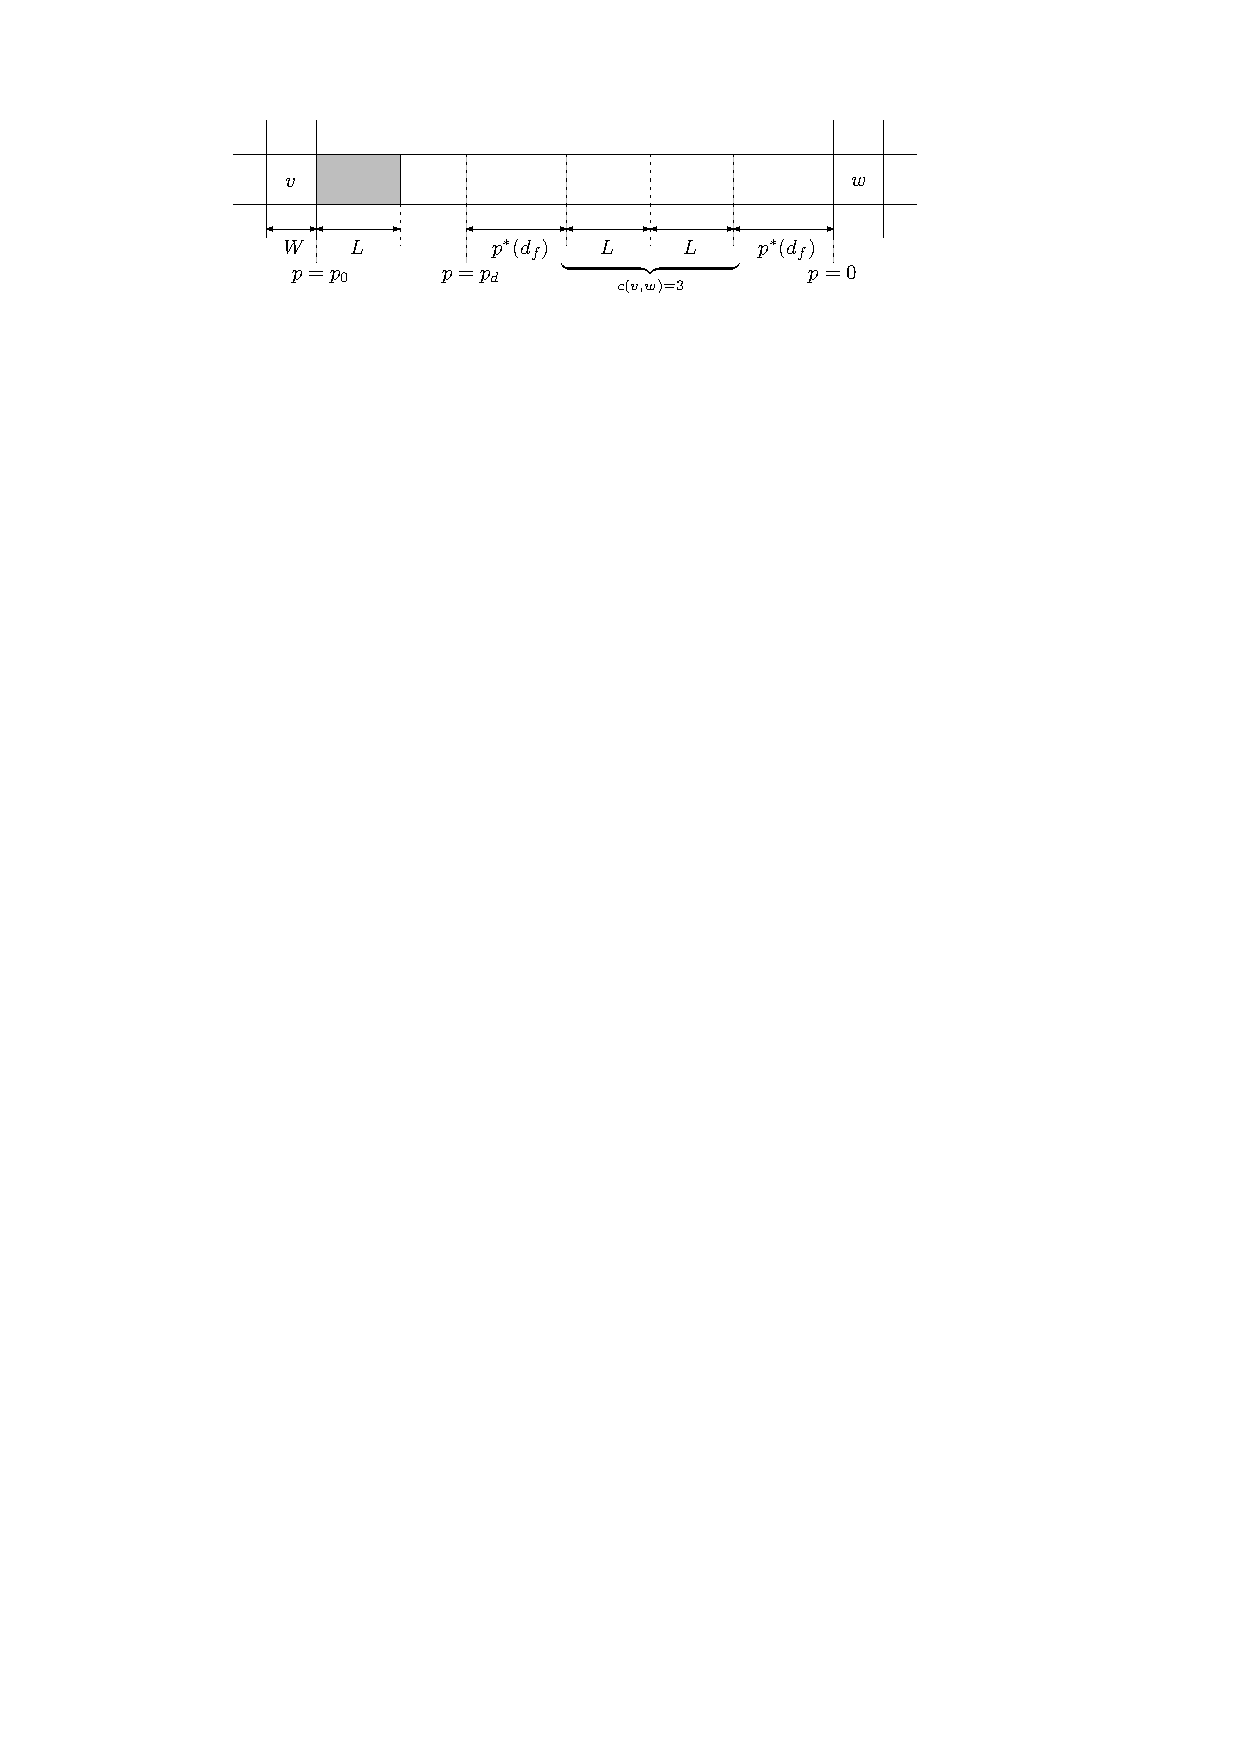
\includegraphics[width=1.0\textwidth]{figures/motion/tandem_annotated}
  }
  \caption{Tandem of intersections with indicated distances used in the capacity
    calculation.}
  \label{fig:tandem_annotated}
\end{figure}

Suppose that we want to design the tandem network such that at least $c(v,w)$
vehicles can enter and decelerate to some waiting position, from which it is
also possible to accelerate again to full speed before crossing $w$.
%
Vehicles are required to drive at full speed $v=v_{\max}$ as long as they occupy
any intersection. Therefore, a vehicle crossing $v$ can only start decelerating
after $x(t) \geq L + W$, so the earliest position where a vehicle can come to a
stop is $x = L + W + x^{*}(T)$.
%
Because vehicles need to gain maximum speed $v=v_{\max}$ before reaching $w$,
the latest position where a vehicle can wait is $x_{f} - x^{*}(T)$.
%
Hence, in order to accomodate for $c(v,w)$ waiting vehicles, the length of the
lane must satisfy
\begin{align}
  d(v, w) \geq L + W + 2x^{*}(T) + (c(v,w) - 1) L ,
\end{align}
as illustrated in Figure~\ref{fig:tandem_annotated}.
%
Conversely, given the lane length $d(v,w)$, the corresponding capacity is given
by
\begin{align}
  c(v, w) = \texttt{floor}\left( \frac{d(v,w) - W - 2 x^{*}(T)}{L} \right) ,
\end{align}
where $\texttt{floor}(x)$ denotes the largest integer smaller than or equal to $x$.

\begin{remark}
  Without Assumption~\ref{assump1}, we cannot derive such a simple expression fo
  the capacity, because it would depend on the specific combination of lengths
  of the vehicles that arrived to the system.
\end{remark}

In order to guarantee feasible trajectories, we need to add capacity constraints
to the crossing time scheduling problem. We are almost sure that it is
\textit{sufficient} to add constraints of the type illustrated in
Figure~\ref{fig:buffer-constraint}. Recall that $\rho = L / v_{\max}$ denotes
the minimum time between two crossing times of vehicles on the same lane. For
every pair of vehicles $i,j \in \mathcal{N}(l)$ such that
$k(i) + c(v,w) = k(j)$, we include the constraint
\begin{align*}
  \bar{t}(y(i, w), d(v, w)) + c(v,w) \leq \bar{t}(y(j, v), 0) ,
\end{align*}
which after substituting the definitions yields
\begin{align*}
  y(i,w) - \frac{d(v,w)}{v_{\max}} + c(v,w) \rho \leq y(j, v) .
\end{align*}
However, we are not sure whether these constraints are \textit{necessary}, i.e.,
there might be situations in which vehicle $j$ is able to cross $v$ slightly
earlier due to the shape of the trajectories.

\begin{figure}[h]
  \centering
  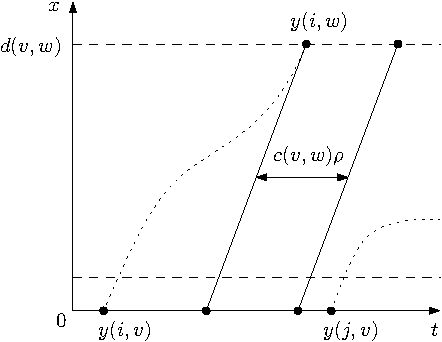
\includegraphics[width=0.6\textwidth]{figures/capacity_constraint.pdf}
  \caption{Illustration of the buffer constraint between $y(i, w)$ and
    $y(j, v)$. The slope of the two parallel lines is $v_{\max}$, so they
    correspond to the schedule times. The two dotted lines are examples of
    trajectories $x_{i}(t)$ and $x_{j}(t)$.}
  \label{fig:buffer-constraint}
\end{figure}


\newpage

\section{Optimal control with state constraints}

We will redefine problem~\eqref{eq:optimal_control} to better fit the common
optimal control notation. In this section, $x(t) = (p(t), v(t))$ will refer to
the \textit{state}, which consists of both the position $p(t)$ and velocity
$v(t)$. It will be more convenient to define the target position $p_{f} = 0$ and
consider the start position $p_{0} = - d(v, w)$, so that the target state is
given by $(0, v_{\max}) = (0, 1)$. The \textit{control} is some function $u(t)$,
which corresponds to acceleration in our particular problem.

\begin{subequations}
\begin{align}
  \min \quad & \int_{t=0}^{T} |x(t)| dt \\
  \text{ s.t. } \;\, & \dot{x}(t) = Ax(t) + Bu(t) , \\
                     & x_{2} \leq 1 , \\
                & x(0) = (-p_{0}, 1) , \\
                & x(T) = (0, 1) , \\
                & {-u_{\max}} \leq u(t) \leq u_{\max} , \\
                & x(t) \leq y(t) ,
\end{align}
\end{subequations}



General form of optimal control with state constraints
\begin{subequations}
\begin{align}
  \max \quad & \int_{t=0}^{T} F(x(t), u(t), t) dt \\
  \text{ s.t. } \;\, & \dot{x}(t) = f(x(t), u(t), t) , \quad x(0) = x_{0} , \\
                & g(x(t), u(t), t) \geq 0 , \\
             & h(x(t), t) \geq 0 , \\
             & a(x(T), T) \geq 0 \\
             & b(x(T), T) = 0 .
\end{align}
\end{subequations}


Linear autonomous optimal control has
\begin{align*}
  f(x(t), u(t), t) = A x(t) + B u(t),
\end{align*}
with $A, B$ constant $n\times n$ and $n \times m$ matrices.

The time-optimal control of a double integrator is often treated as example in
introductory texts on optimal control theory. However, our problem differs from
this version in the following ways:
\begin{itemize}
  \item We have a fixed terminal time $T$.
  \item The safe following constraints are state constraints.
  \item Target state is $(p(t), v(t)) = (0, 1)$.
\end{itemize}


\end{document}
